\documentclass{beamer}
\usepackage[english]{babel}
\usepackage[utf8]{inputenc}
\mode<presentation>{\usetheme{FS18}}
\usepackage{amsmath,amsthm, amssymb, latexsym}
\usepackage[orientation=portrait,size=a0,scale=1.4]{beamerposter}
\usepackage{natbib}
\bibliographystyle{unsrt}
\usepackage{subcaption}
\graphicspath{{../figures/graphics/}}
 
\title{Local Variance Optimization for the Autonomous Regulation of Echo State Networks}
\author{Fabian Schubert, Claudius Gros}
\institute{Institute for Theoretical Physics, Goethe University Frankfurt a.M.}
\date{}

\renewcommand{\vec}[1]{\mathbf{#1}}

\newcommand{\vx}{\vec{x}}
\newcommand{\vy}{\vec{y}}
\newcommand{\vf}{\vec{f}}
\newcommand{\vsigm}{\boldsymbol{\sigma}}

\newcommand{\Err}{\mathrm{Err}}
\newcommand{\Exp}{\mathrm{E}}
\newcommand{\Var}{\mathrm{Var}}

\newcommand{\avgt}[1]{\left< #1 \right>_T}
\newcommand{\avgp}[1]{\left< #1 \right>_P}


\begin{document}
\begin{frame}[t]
\begin{columns}[t]
\begin{column}{.4\textwidth}
\begin{myblock}{Introduction}
\begin{itemize}
	\item Echo state networks have proven to be a powerful tool in the field of time series prediction~\citep{Jaeger_2001}.
	\item Several approaches to the optimization of the dynamic reservoir have been investigated in the past, including global tuning for criticality~\cite{Livi_2016}, as well as local adaptation towards a given output distribution~\cite{Schrauwen_2008}.
	\item The spectral radius $|\Lambda_{\rm max}|$ of the synaptic weight matrix provides a measure to regulate the network in an appropriate working regime~\cite{Caluwaerts_2013}. We show that $|\Lambda_{\rm max}|$ can be regulated by local homeostasis of the variance $\sigma_y^2$ of neural activity. This variance control operates on the gain of the neural transfer function and its optimization target depends on the variance $\sigma_{\rm ext}^2$ of external input.
	\item In contrast to previously proposed optimization rules via local intrinsic plasticity, our model relies on the assumption that external and recurrent input signals can be treated as two separate streams of information. The network can hence react autonomously to changes of the input statistics.
\end{itemize}
\end{myblock}

\begin{myblock}{Model Description}
\begin{align*}
y_i^{t+1} &= \mathrm{tanh}\left( a_i^t I_i^{t+1} \right) \\
I_i^{t+1} &= \sum_{j=1}^{N} W_{ij} y_j^t + E_i^{t+1}  \\
b_i^{t+1} &= b_i^t + \epsilon_{b} \left[ \avgt{y_i} - \mu_{t} \right] \\
a_i^{t+1} &= a_i^{t} + \epsilon_{a} \left[ \sigma_{t}^2 - \left( y_i^t - \overline{y}(t)_i\right)^2 \right]  \\
\overline{y}^{t+1}_i &= \epsilon_{\rm trail} \left[ y_i^{t+1} - \overline{y}^{t}_i\right]
\end{align*}
\begin{itemize}
	\item $W_{ij}$ is a sparse random matrix with connection probability $p$. Nonzero entries were drawn from a Gaussian distribution $\mathcal{N}(\mu = 0,\sigma = 1/\sqrt{N p})$. Diagonal entries were always set to zero.
	\item $E^t_{i}$ are random vectors of size $N$ with independent entries drawn from a Gaussian distribution $\mathcal{N}(\mu = 0,\sigma = \sigma_{\rm ext})$.
	\item By changing individual gain and bias values $a_i$ and $b_i$, the homeostatic control tries to drive the activity standard deviation and mean of every cell to the value given by $\sigma_{t}$ and $\mu_{t}$.
\end{itemize}
\vspace{20pt}
\begin{figure}
	\centering
	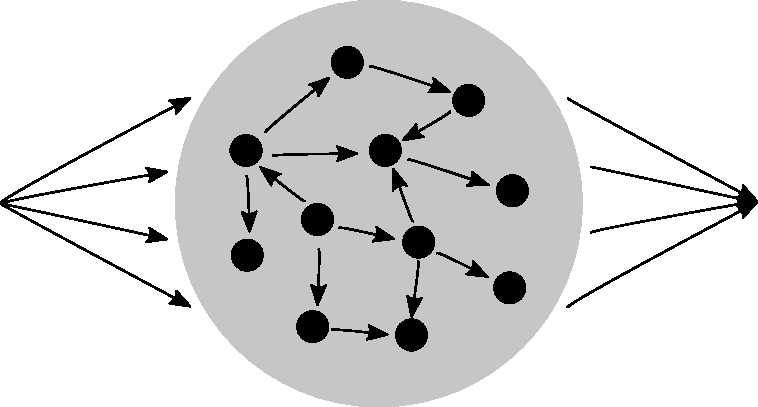
\includegraphics[width=0.7\textwidth]{../figures/illustration.pdf}
\end{figure}
\begin{itemize}
	\item By controlling the output variance of the neural activity, we can tune the network into a regime that exhibits subcritical, but transiently active dynamics in the absence of external input.
	\item This led to the question how a homeostatic variance control could be used to tune network properties into a desired regime, even under changing input statistics.
	\item In particular, we were interested in the relation between target variance and the variance of the external signal with respect to optimal memory capacity and a critical boundary of the so-called \textit{echo state property} \cite{Jaeger_2001}. 
\end{itemize}
\end{myblock}

\begin{myblock}{Self-Consistency Equation}
	If we assume no correlations in time across the neural population, we can formulate a self-consistency equation, given by
	\begin{equation*}
	\sigma^2_{t} = \int_{-\infty}^{\infty}  \tanh^2\left(ay\right) \mathcal{N}\left(y, \mu = 0, \sigma = \sqrt{\sigma^2_{t} + \sigma^2_{\rm ext}}\right)	\mathrm{d}y \;. 
	\end{equation*}
	
	As a second order approximation with respect to $\tanh$, we can use $\tanh^2(y) \approx y^2 - \frac{2}{3} y^4$ in the integral, which gives
	
	\begin{align*}
	\sigma_{t}^2 &\approx \frac{1}{a\sqrt{2 \pi}\sigma_{\rm total}}\int_{-\infty}^{\infty}\left( y^2 - \frac{2}{3}y^4\right)\exp\left( \frac{-y^2}{2a^2\sigma_{\rm total}^2}\right) \mathrm{d}y \\
	&= a^2\sigma_{\rm total}^2 - 2a^4\sigma_{\rm total}^4 \\
	&= a^2\left( \sigma^2_{t} + \sigma^2_{\rm ext} \right) - 2a^4 \left( \sigma^2_{t} + \sigma^2_{\rm ext} \right) \; .
	\end{align*}
	This approximate solution is shown in Fig.~\ref{fig:sweep_sim}B.
\end{myblock}

\begin{myblock}{Optimal Memory Capacity}
	\begin{itemize}
		\item We determined the memory capacity of the ESN after homeostasis has equilibrated for different pairs of input and target variances, see Fig.~\ref{fig:sweep_sim}D.
		\item Given that the transition shown in Fig.~\ref{fig:sweep_sim}B bears a similar functional relationship between $\sigma_{\rm ext}$ and $\sigma_t$, we would like to further investigate the possibility of a local homeostatic control that optimizes MC based on the second moments of the neural activity itself and the external input. 
	\end{itemize}
\end{myblock}

\end{column}

\begin{column}{.55\textwidth}
\begin{myblock}{Network Dynamics}
	\begin{figure}
		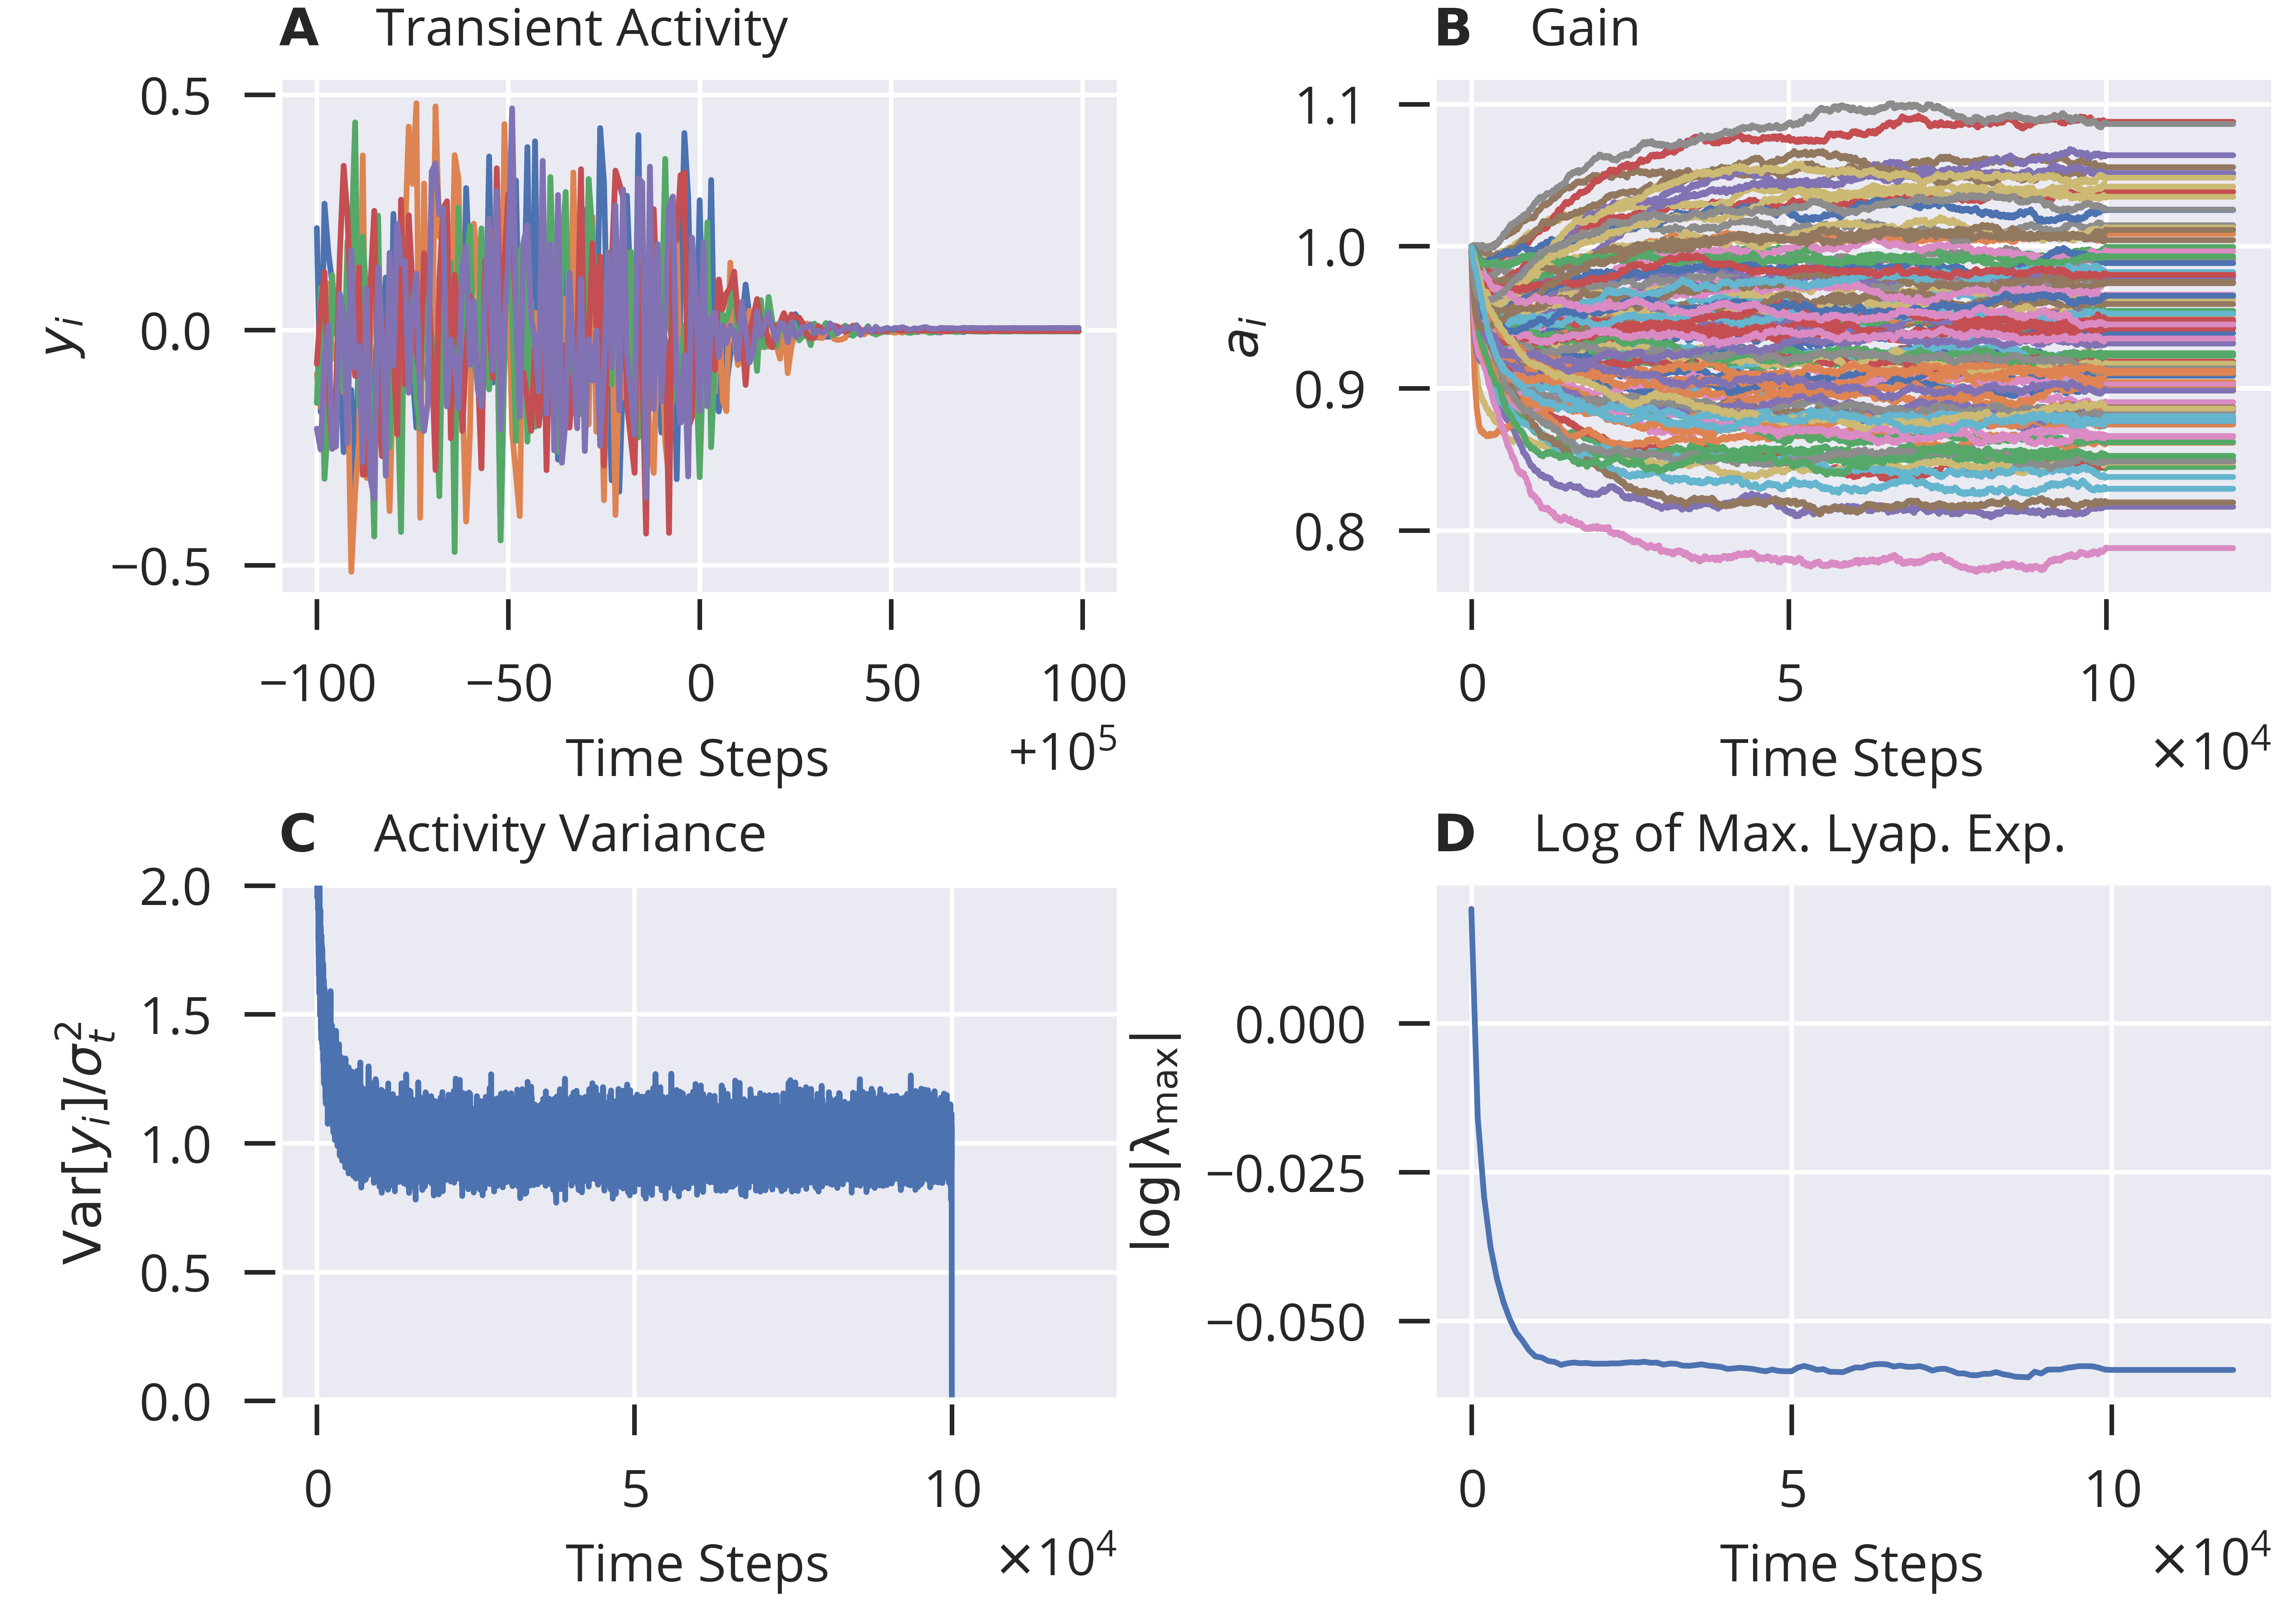
\includegraphics[width=\textwidth]{../figures/res_comp.png}
		\caption{Exemplary network dynamics, where the external input was switched off after $10^5$ time steps, followed by a transient period of decaying activity.}
		\label{fig:trans_dyn}
	\end{figure}
\end{myblock}	

\begin{myblock}{Changing Input and Target Variance}
\begin{itemize}
	\item In the absence of external input, a spectral radius of $|\Lambda_{\rm max}| = 1$ denotes a boundary between contracting and chaotic dynamics. We determined the shape of this transition in the $\left(\sigma_{\rm ext},\sigma_t\right)$ space.
\end{itemize}
	\begin{figure}
		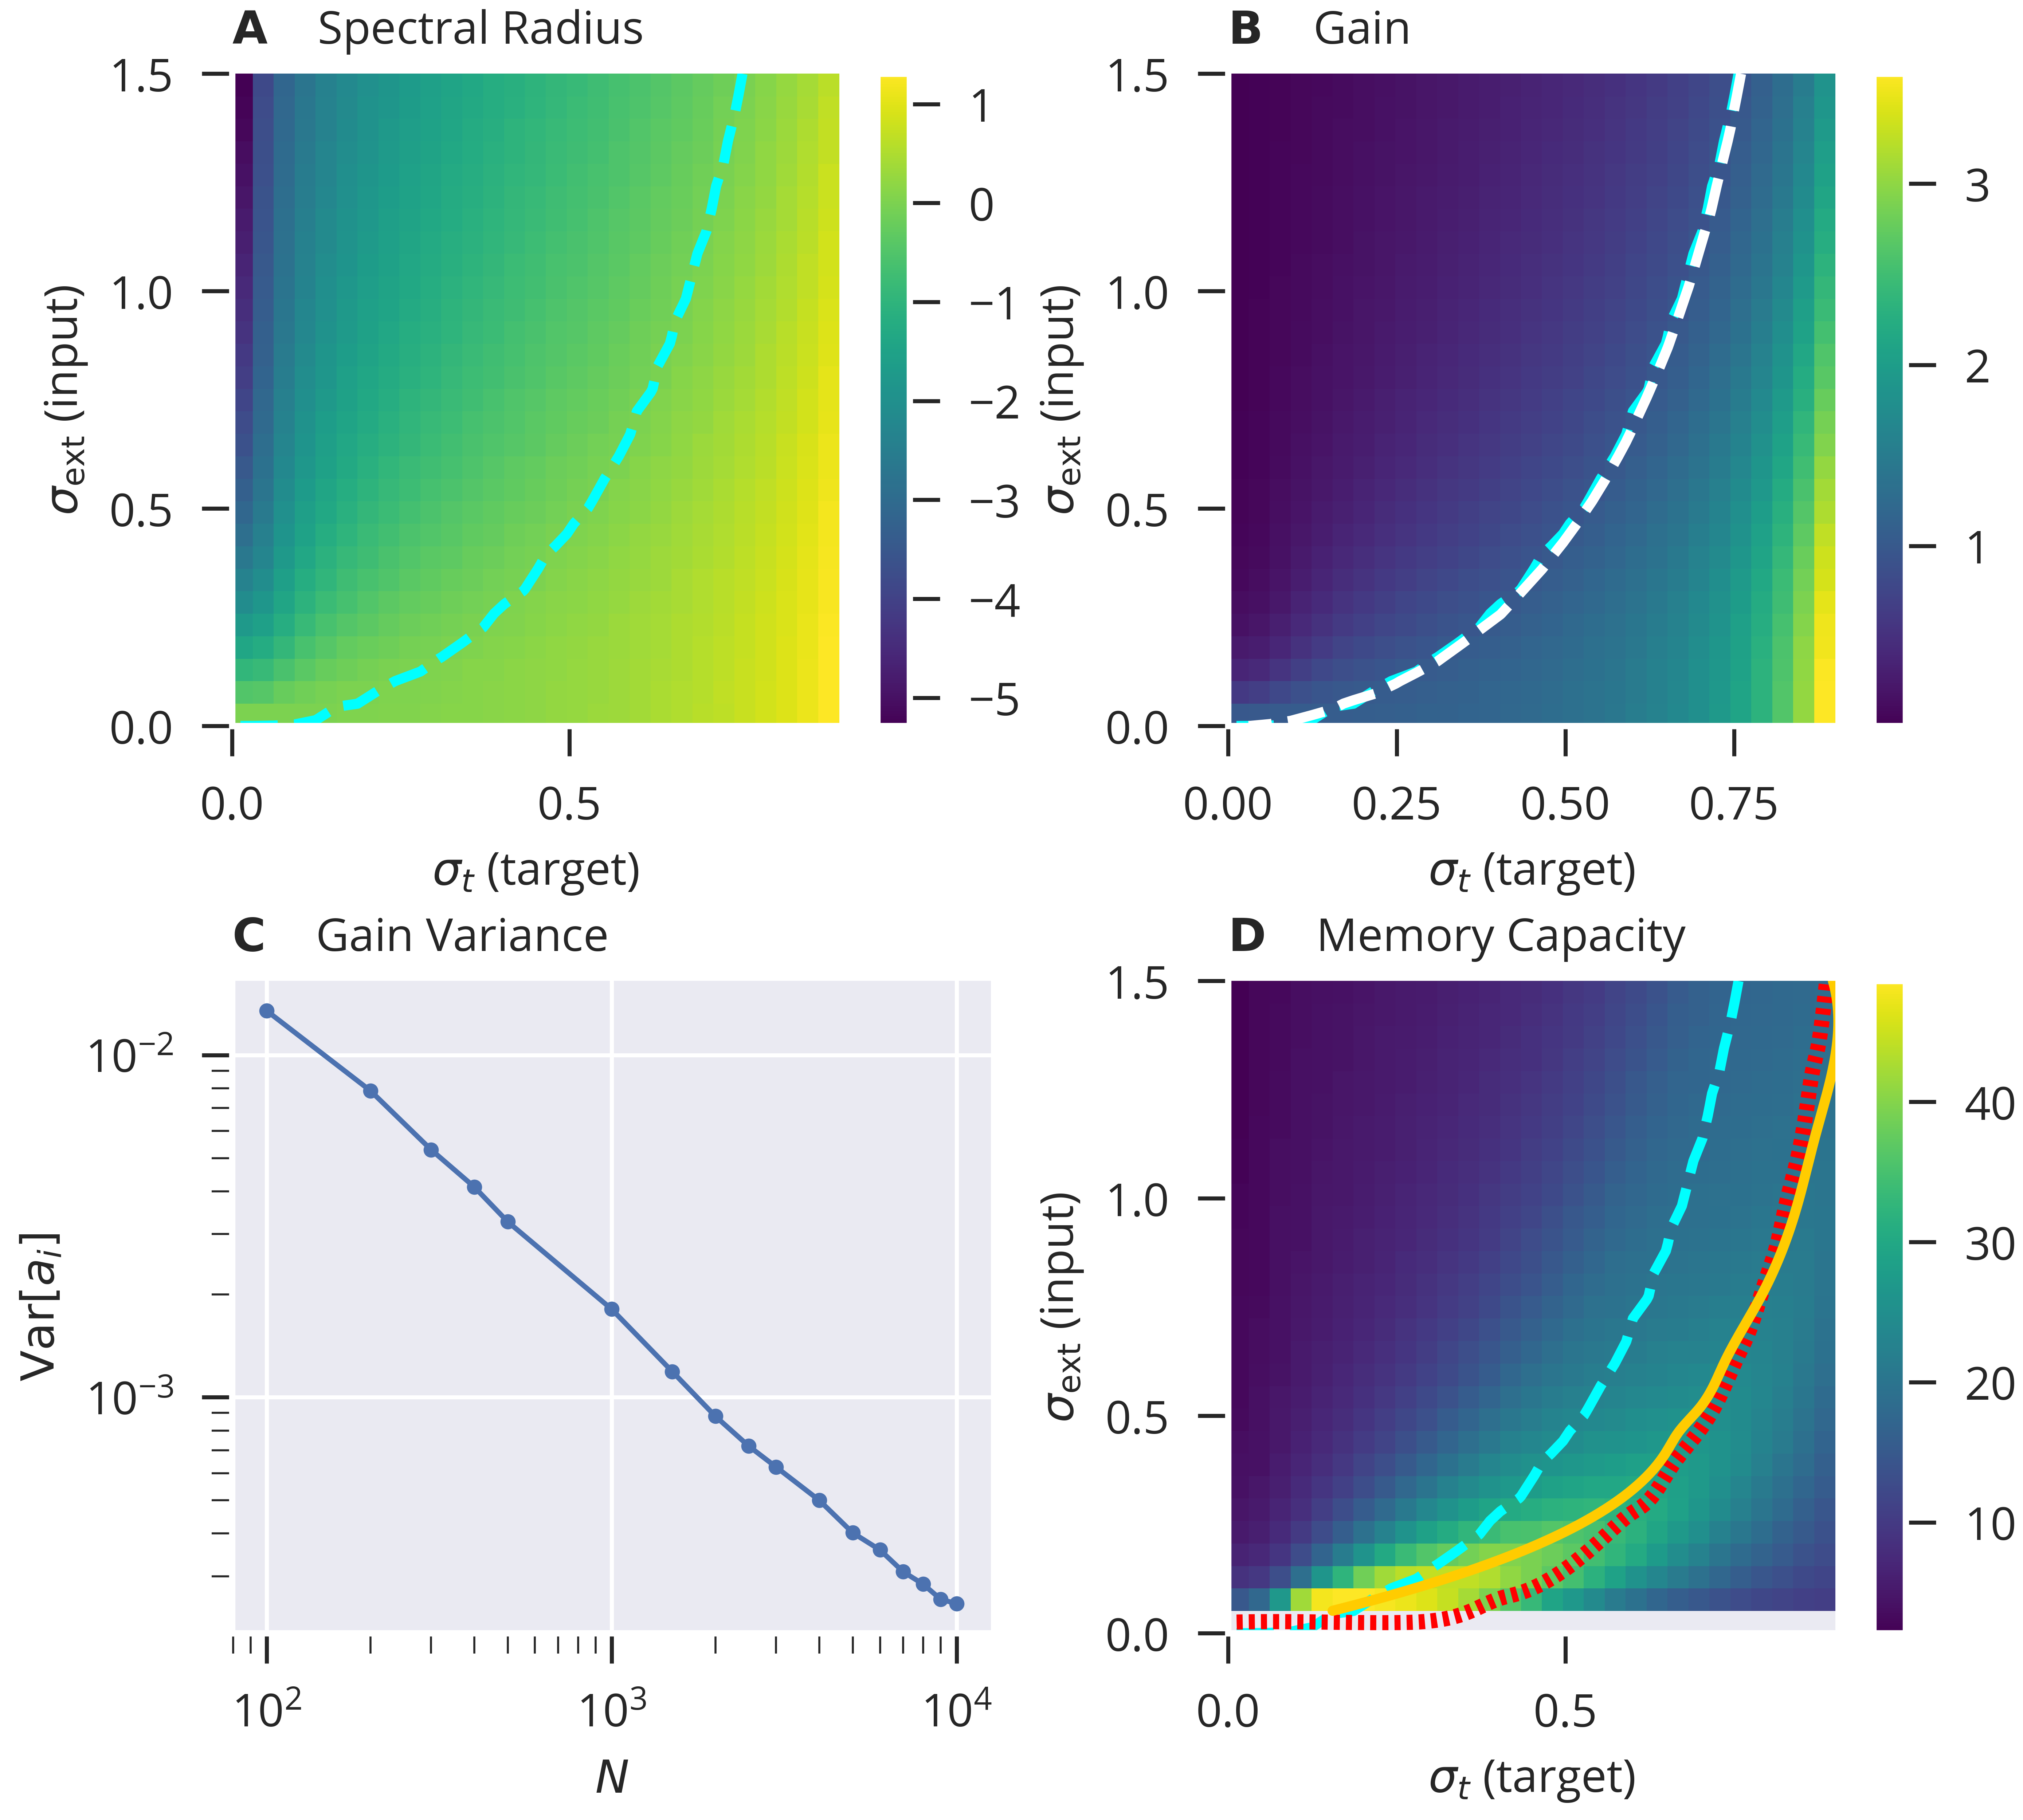
\includegraphics[width=0.9\textwidth]{../figures/std_in_std_target_sweep_fig.png}
		\caption{(A): Spectral Radius of $a\cdot W_{ij}$, where the line marks $|\Lambda_{\rm max}| = 1$. (B): Gain values, with $a=1$ marked by white line. Blue line as in (A). Yellow line is a second order approximation of the transition. (C): Gain variance over population converges to zero for large network sizes. (D): Memory capacity (MC), yellow line marks max. MC for a given $\sigma_{\rm ext}$, red line the loss of the echo state property. Dashed line as in (A).}
		\label{fig:sweep_sim}
	\end{figure}
\end{myblock}


\begin{myblock}{References}
	\scriptsize
	\bibliography{../../../../../lit_base.bib}
\end{myblock}

\end{column}
\end{columns}
\end{frame}
\end{document}
